\documentclass[12pt,oneside,abbrevs,dtc,mscres,neuro,notimes,logo]{styles/infthesis}

% Packages
\usepackage{graphicx}
\usepackage{abbrevs}
\usepackage{acronym}
\usepackage{minted}
\usepackage{multirow}
\usepackage{wrapfig}
\usepackage{cite} 
\usepackage{gensymb}
\usepackage{amsmath}
\usepackage{mathtools}
\usepackage{tikz}
\usepackage{pgfplots}
\usepackage{scalefnt}
\usepackage{subfig}
\usepackage{tabularx}
%\usepackage{subcaption}
\usepackage{array}
%\usepackage{pgffor,pgf}
\usepackage{biblatex}
\usepackage{psfrag}
\usepackage{lipsum}
\usepgflibrary{plothandlers}
\usetikzlibrary{plotmarks}
\pgfplotsset{compat=newest}

%adding path to images
\graphicspath{{./images/}}

%alias cite to autocite, cites to autocites

\mathtoolsset{showonlyrefs=false}

\renewcommand\theFancyVerbLine{\normalsize\arabic{FancyVerbLine}}

% Project Details
\title{Title Pending}
\author{Gavin Gray}
\submityear{2014}
\date{\today}

%Hofstadter's Law: It always takes longer than you expect, even when you take into account Hofstadter's Law.
%
%— Douglas Hofstadter, Gödel, Escher, Bach: An Eternal Golden Braid
%
% obligatory spell/etc check reminder
% go through for acronym/symbols at end
%
% Pending:
%
% * Background
%   * Intro
%   * Protein complexes and community detection
%

%%\newacro{ACRNM}{Description}
\newacro{DIP}{Database of Interacting Proteins\autocite{xenarios_dip_2002}}
\newacro{HIPPIE}{Human Integrated Protein-Protein Interaction rEference\autocite{schaefer_hippie:_2012}}
\newacro{PPI}{Protein-Protein Interaction}
\newacro{SVM}{Support Vector Machine}
\newacro{STRING}{Search Tool for the Retrieval of Interacting Genes/Proteins}
\newacro{AUC}{Area Under Curve}
\newacro{ROC}{Receiver Operating Characteristic}
\newacro{PIPs}{(Human) (Protein-)Protein Interaction Predictions}
\newacro{PCA}{Principal Components Analysis}
\newacro{RBF}{Radial Basis Function}
\newacro{KDE}{Kernel Density Estimation}

\abstract{
    This project focuses on the synaptic active zone network defined through experiments performed as part of the SYNSYS collaboration.
    Diverse data sources were used to appropriately weight the edges using a combination of a supervised binary classifier and a manually adjusted Naive Bayes model.
    A spectral modularity community detection algorithm was used to produce two sets of communities from the weighted and unweighted cases.
    The resulting communities were then compared using \ac{NMI} and in terms of disease association.
    Communities detected and disease associations within these differed between the weighted and unweighted cases.
}


% Extra Package Commands

\begin{document}
  \begin{preliminary}
    % Title Page
    \shieldtype{1}
    \maketitle

    % Preamble
    \begin{acknowledgements}
    %to be included:
    % Colin
    % Finlay
    % Danilo (for the template)
    % Biological databases

    \lipsum[1-2]

\end{acknowledgements}

    \standarddeclaration
    \input{sections/misc/dedication}
    \tableofcontents
    \listoffigures
  \end{preliminary}

  % Chapters
  \chapter{Introduction}
\label{introduction}

%intro to the intro here


\section{Motivation}

%expanded version of the above? need stats on depression and schizophrenia
It is estimated that disorders of the brain cost Europe €798 billion Euros in 2010\autocite{olesen_economic_2012}.
Specifically, depression is estimated to cost Europe €91.9 billion in 2004 and schizophrenia along with associated psychotic disorders is estimated at €93.9 billion.
There are many diseases with limited treatment options in the brain, and a deeper understanding of the brain is required to treat them. 

%FIN: even in motivation say why proteins matter to understanding brain - key components, molecular machines etc

These diseases are very likely to act at the synaptic level\autocites{chua_architecture_2010,synsys}.
However, the exact proteins or genes involved in these diseases are unknown.
If it is possible to even gain slightly more information about associated proteins at the synapse it may be possible to develop new treatments\autocite{li_interaction_2010}.

In addition, as a project this includes work from various areas, such as Bioinformatics, Machine Learning and Software Development that made it a good learning exercise. %FIN: thus made it a good 
It is a worthwhile investment in the fundamentals of constructing \ac{PPI} networks. %FIN: first usage of acronym should be in full, Protein-Protein Interaction 

%overview of the project or the report? pretty sure it's the report
\section{Outline}
%sections to cover:
% background
% methods
% results
% conclusion

This project involved combining both direct and indirect data sources to create weighted edges in a \ac{PPI} graph to affect the communities detected by a Community Detection algorithm.
A flow chart describing this process and the elements involved is shown in figure \ref{fig:expflow}.
There are three main input sources shown, the pull-down experiments, direct data and indirect data.
%FIN: worth briefly explaining what pull-down experiments are or their importance i.e. that they are potentially empirical molecular validation of protein-protein interaction predictions
Pull-down experiments were used to identify the proteins of interest, which were used to build an interaction network using direct data sources, such as interaction databases.
The indirect data sources, such as functional annotations of proteins, were used along with direct data sources in the process to generate weighted graphs.

%flow charts from the proposal could go here
\begin{figure}
    \centering
    \includegraphics[width=0.6\textwidth]{expflow.png}
    \caption{A flow chart describing how the elements of the project as a whole, as shown in the project proposal.}
    \label{fig:expflow}
\end{figure}

The resulting weighted and unweighted \ac{PPI} graphs were then separated into communities using a Community Detection algorithm.
These communities could then be compared using the two methods named in figure \ref{fig:expflow}: Disease Enrichment and NMI.
The results of these tested the hypothesis of the project. %FIN: "results of these were used to test" is clearer

%hypothesis required %FIN: hypothesis needs stated earlier - this is a bit confusing
The hypothesis of this project was that the communities detected in each case would differ and that these differences would be relevant to the conclusions each network could illustrate about a particular disease.
NMI was able to show simply that the two sets of communities detected was different. %FIN: were different
Disease enrichment refers to testing the likelihood that a given community is involved in a particular disease. %FIN: for example? You would expect a community to represent a certain cluster of interacting proteins right? 
%FIN: they identify a high confidence interaction network/cluster around known Alzheimer's related proteins and identify putative additional factors  Genome Res. 2011 Mar;21(3):364-76. doi: 10.1101/gr.114280.110. Epub 2010 Dec 16.
%FIN: Interactome mapping suggests new mechanistic details underlying Alzheimer's disease.
%FIN: Soler-López M1, Zanzoni A, Lluís R, Stelzl U, Aloy P.
This allowed us to show the differences in the predictions for disease involvement given by each network due to the weighting of the networks.
%FIN:this sentence is horrific - split it or rephrase

%structure of the report and other resources
The report first describes the background knowledge driving the hypothesis of the project in chapter \ref{background}.
In chapter \ref{methods} the methods involved in executing the project are described.
Finally, the results obtained are described in chapter \ref{results}.
In addition, the execution of all commands required to reproduce the project were recorded in notebooks described in section \ref{app:notebooks}.
This project was stored in a git repository and is publicly available in a repository described in Appendix \ref{app:repository}.

%progress flow charts from the proposal could go here, or above

%could also include one updated to reflect the real project

%should also mention the prototype run through and which week it occurred in 

\section*{Conclusion}

The following report covers the background information necessary to understand the methods of the project and the results which were obtained.
It was approached as an opportunity to use a variety of new tools, and each will be described as the report continues. %FIN: "an opportunity to investigate the effectiveness of new tools in resolving known issues in predicting \ac{PPI}" or something like that

  \chapter{Background}
\label{background}

%intro to background
This project involved the use of protein interaction prediction to build weighted \ac{PPI} networks improve the performance of Community Detection on a \ac{PPI} network for disease research.
The following chapter describes the relationship of the disease to the proteins of the synapse.
\ac{PPI} networks, and their application to disease research is then described.
%FIN: I'd probably explain the \ac{PPI} acronym once more for people that skipped the beginning
%The aim of the Community Detection algorithm was to gain insight into structure of the interactions between proteins at the synapse to aid disease research.
%FIN: you need to justify why the synapse is important in neuronal disease research with a reference at least
%In the following chapter these different components, and how they fit together, will be described.

%what is a protein-protein interaction network?
\section{The synapse and protein interaction}

%intro paragraph, why proteins are important
Proteins consist of approximately 20\% of cell mass in a typical eukaryote\autocite{lodish_molecular_2000}.
%FIN: quantify - account for ~20% of the cell mass of a "typical eurkaryote" http://www.ncbi.nlm.nih.gov/books/NBK21473/
%FIN: "synthesis of proteins accounts for a considerable if highly variable proportion of the normal metabolism of a cell"  http://www.sciencedirect.com/science/article/pii/S1574789109000751
Each of these proteins are molecules which fit into machinery of a cell within the human body.%FIN: I dislike this sentence from an evolutionary perspective - plenty are shit - "Proteins facilitate almost every aspect of cellular metabolism across all forms of life.  They have evolved complex and extensive systems of interaction with one another and other cellular macro and micromolecules"
Functions of these cells include almost all cellular functions; there are proteins capable of pumping ions, reshaping DNA and fluorescing\autocite{alberts_molecular_2008}. %FIN:shoulda read the next sentence first before writing the last comment... still change that last 'tuned' sentence
A crude model of the cell is to map the interactions between these molecular machines to try to guess about the functioning of the cell. %FIN: explain why this is crude - it ignores the interaction of proteins with everything else!
These models are \ac{PPI} networks and can be useful for targeting proteins in disease research\autocite{chen_identifying_2013}. %FIN: expand a little: how are they useful?  They allow targeted research, can identify additional previously uncharacterised disease factors, are targets for molecular therapies add a reference to one of the many \ac{PPI} papers you are citing that explain why \ac{PPI}s matter 

%what are synapses?
Synapses are the contacts between nerve cells where the vast majority of communication between nerve cells occurs, the only exceptions being through signalling molecules that can cross the cell membrane as shown in figure \ref{fig:actzone}.
There are two types of synapses in the nervous system, electrical and chemical\autocite{kandel_principles_2000}.
Electrical synapses form a simple electrical connection through an ionic substrate between two neurons.
Chemical synapses are involved in a much more complex system of neurotransmitter release and reception.
Synapses are therefore important to the functioning of the nervous system. 
A problem with synapse function will likely cause large problems to the nervous system, so diseases of the nervous system are likely to involve problems with synapse function. %FIN: use the word neurotransmission its a great word, bonus points for 'impinge' 
%As the cell is composed of proteins, so is the synapse composed of proteins. %FIN: there are lots of other shit too - I'd get rid of this its too simple in this form.  "As synapse function heavily features the interaction of many proteins e.g. transporters, signal-receptors, ... etc" - maybe choose some random specific examples
Investigating the functioning of these proteins will help to explain the functioning of the synapse and hopefully provide insight into the diseases of the synapse\autocite{synsys}.%FIN:such as?  Some autistic spectrum disorders have been connected with heritable loss-of-function mutations in synaptic regulatory proteins such as Neuroglobin 4 http://jp.physoc.org/content/587/4/727

%going deeper, why do we care about proteins at the synapse, mention SYNSYS
The proteins at the synapse drive synaptic communication, which in turn defines the functioning of the brain.  %FIN: explain what the synapse is- the princpial interaction interface of a neuron - maybe move synapse section to before where yout alk about it
As these proteins define the functioning of the brain any disorders which affect the brain are very likely to involve these proteins.  %FIN: doesn't really justify why \ac{PPI} itself is important though
Disorders which affect the brain are also very common and poorly understood, affecting one in three people in the developed world. %FIN: \ac{PPI} offer opportunities to use known factors to identify additional uncharacterised protein factors in neuronal diseases
Curing these diseases therefore may be possible through a greater understanding of the interactions of proteins at the synaptic level\autocites{synsys,chua_architecture_2010}.

%but what is a protein-protein interaction network?
Physical interaction between proteins can be inferred from a range of different experiments.
Typical contemporary protein interaction networks rely on databases of confirmed interactions from a variety of experiments, for example in \textcite{kenley_detecting_2011} several well-known interaction databases were used, such as BioGRID\autocite{stark_biogrid:_2006}. %FIN:give an example of one or two e.g. \ac{DIP} and BioGRID 
By forming a network from these individual interactions as edges and clustering this network \textcite{kenley_detecting_2011} were able to predict complexes and functional associations. %FIN: example paper doesn't sound quite right - "Kenley et al. were able". Be more specific in what a functional association is
As with functional association, through associating community members with disease it is possible to associate communities with diseases, as will be discussed in chapter \ref{methods}. %FIN:how? If members of this functional association has been previously implicated in diseases or something

%historical work in the field
Two papers, \textcite{ito_comprehensive_2001} and \textcite{uetz_comprehensive_2000}, were able to leverage large volumes of recent interaction data and build interaction networks. % mention they collected a lot of their own data in earlier papers by molecular methods (yeast-2h)
These papers were able to make interesting discoveries about the network of interactions in yeast simply by investigating subnetworks in the network that was produced.  %FIN: for example? identification of many previously unidentified proteins involved in yeast vesicular transport such as Ygl161c, Ygl198w, and Ylr324w

%which network are we interested in and stating the aims of the project
The aim of this project is to extend work in the field of protein interaction prediction \autocites{qi_evaluation_2006,mcdowall_pips:_2009,rodgers-melnick_predicting_2013,von_mering_string:2005} to weighting protein interactions with a posterior probability through the use of varied data sources.
Specifically, the interactions we are considering are those of the active zone network illustrated in figure \ref{fig:actzon} found as part of the SYNSYS project\autocite{synsys}.
This data forms a set of proteins and a prepared unweighted list of protein interactions summarised in table \ref{tab:synsys}.
These proteins and their interactions were found through immuno-precipitation, or pull-down, experiments in the mouse hippocampus focusing on the pre-synapse.
In these experiments a set of bait proteins are selected and used to attract a set of prey proteins, the interaction between bait and prey being the interactions detected.
The exact set of interactions used in the unweighted network used was prepared prior to this project using additional resources: HIPPIE\autocite{schaefer_hippie:_2012}, InterologWalk\autocite{gallone_bio::homology::interologwalk_2011}, BiGRID\autocite{stark_biogrid:_2006}, CCSB\autocite{yu_high-quality_2008}, HPRD\autocite{baolin_hprd:_2007}, IntAct\autocite{hermjakob_intact:_2004} and MDC\autocite{futschik_comparison_2006}.
%The interaction network we are investigating in this work is referred to throughout as the active zone network in the synapse.
%These proteins are part of the pre-synapse and are illustrated in figure \ref{fig:actzone}.
%Proteins identified as part of this network were used as baits in the pull-down experiments whose results are used in this project to build the \ac{PPI} network which is the focus of the weighted and unweighted Community Detection.
%FIN: what is a pull-down experiment you still haven't explained it or why it is 'gold-standard' or that it is one of the gold-standards for demonstrating \ac{PPI} in-vitro. Life scientists love to differentiate between in-vitro and in-vivo. While pull-down experiments can show interactions in-vitro (i.e. a test-tube) it doesn't necessarily mean the cells will interact in-vivo (in the cell).  That is why demonstrating that two proteins that interact also co-localise in the cell is important to confirm functional interaction.  Cells, and especially eukaryotic cells aren't really big bags of proteins (and other molecules) as they are often drawn in books - they contain a complex set of compartmentalisation, diffusion gradients and active retention or inactivation of proteins in certain areas

\begin{figure}
    \centering
    \includegraphics[width=\textwidth]{actzone.png}
    \caption{An illustration of the proteins identified to be involved in the active zone network\autocite{chua_architecture_2010}.}
    \label{fig:actzone}
\end{figure}

%synsys table: no. of baits, preys, interactions, etc?
\begin{table}
    \centering
    \begin{tabular}{l c c} 
        \multicolumn{3}{*}{Number of} \\
        baits   & preys & interactions \\
        \hline
        24      & 1548  & 9372 \\
    \end{tabular}
    \caption{A table summarising the results of the pull-down experiments performed as part of the SYNSYS project\autocite{synsys}, and the active zone network defined using them, used in this project.}
    \label{tab:synsys}
\end{table}

%function of the active zone network? What does it do?

%what is community detection?
\section{Protein complexes and community detection}

As mentioned in the previous section it is possible to analyse \ac{PPI} networks to detect protein complexes and functional groups. %FIN: to identify predict \ac{PPI} - unless you have proper co-localised interaction you can't say for certain they interact 
This has recently been achieved through use of Community Detection\autocites{chen_identifying_2013,wang_recent_2010}, which uses various methods to find community structure in graphs.

%what is community structure?
Community structure is described as a characteristic of graphs which have many connections within sub-groups but few connections outside that group\autocite{newman_communities_2012}.
Unfortunately, this description is not specific on exact measures for a graph to have community structure. %FIN: a little flippant - the specific criteria for a community in a graph is an open topic of discussion in the literature or something
Community detection algorithms are simply tested on graphs that are agreed to exhibit community structure with the aim of finding the pre-defined communities. %FIN: by whom, cite an example of one of these test graphs 

%describe how these algorithms usually work
Two important approaches to the problem of Community Detection are traditional hierarchical methods and more recent optimization based methods\autocite{newman_communities_2012}.
Hierarchical methods were developed in the field of sociology and involves grading nodes by how highly connected they are in the network and then using this value to group nodes into communities.
Optimization based methods involves, such as spectral modularity, involves grading edges and removing them iteratively to reveal the community structure.
%a different measure known as betweenness, which is analogous to the current flowing along edges if the graph were an electric circuit, and then allows a reductive technique where edges are removed iteratively to reveal sub-graphs without connections between them. %FIN:sentence needs fixed/split it too complex

%example paper using community detection on ppi graphs?
%FIN: http://www.biomedcentral.com/1752-0509/4/100/ 

%what is protein-protein interaction prediction?
\section{Protein-protein interaction prediction}

Protein interaction prediction was developed to solve the problem of incomplete and unreliable interaction data by combining both direct and indirect information\autocite{qi_learning_2008}.
Direct information are the result of experiments, such as yeast two-hybrid, intended to directly find protein-protein interactions.  %FIN: explain what y2h is and why it is good - you reconstitute some split marker (transcription factor or something) only when two proteins interact from 2 genetically modified yeast hybrids. So if you see that marker it means that the proteins you've put in each hybrid interact
Indirect information includes biological data that was not gathered directly to find interactions, such as gene expression data. %FIN: explain; two proteins can only interact if they are both expressed at the same time and place within a cell therefore co-expression and co-localisation data are important sources of indirect evidence for \ac{PPI} (in fact are necessary for true \ac{PPI})

%what are features?
To predict a protein interaction we need to have a value or sequence of values from which to make our guess as to the existence of an interaction.
For each interaction this set of values are known as features.
The bulk of this project, described in chapter \ref{methods}, involved obtaining these values for every feature necessary to train the classifier and classify the interactions of the synaptic network.  %FIN: maybe expand on this being non-trivial due to the plethora of data sources and alternative identifiers they use. 

%what is the classifier
The classifier, or model, is a machine learning algorithm that can learn from a labelled training set how to sort these vectors of features into the appropriate category. %citation to Murphy?  %FIN: citation to the Murphy's law might be appropriate... 
However, these algorithms cannot make predictions unless the training data is informative.   
Also, the training data must be an accurate representation of the case the algorithm is planned to be applied to. %FIN:make this specific to your data as well - so for example the training data must use validated examples of protein protein interactions 

%why do we want to predict protein-protein interactions?
%reference to ENTS and similar projects aiming to make full interactomes
%how this is different to our goal
Completing the interactome of a given organism from incomplete data is a major goal for some works in the protein interaction field, such as \textcite{rodgers-melnick_predicting_2013}.
The goal in this project is to appropriately weight interactions in a \ac{PPI} network to improve the performance of a Community Detection algorithm.

%what's the point in weighting connections?
Weakly interacting proteins will have a lower confidence in their interacting at all, as it will have been observed less frequently.
Therefore, by weighting the interactions in a \ac{PPI} network according to our confidence we can also make the \ac{PPI} network reflect more closely the true interactions existing in vivo. %FIN: i.e. proteins predicted to interact actually interacting in vivo 

%what data sources were used to predict protein-protein interactions?
\section{Data sources and networks}
\label{back:sources}

%Different types of sources used with reference to other works
Many different data sources were considered for inclusion in this project. %FIN: such as - which ones haven't been mentioned in the table - that you considered but discarded 
The full list can be found in Appendix \ref{datasources}.
These different data sources fall into categories described in table \ref{tab:sources}, while the results of the SYNSYS pulldown experiments can be found in table \ref{tab:pulldown}.

\begin{table}
    \centering
    \small
    \begin{tabular}{p{0.2\textwidth} p{0.5\textwidth}}
        Data source type                                & Examples \\
        \hline
        \multirow{3}{*}{\parbox{0.2\textwidth}{Primary interaction databases}}  & \ac{DIP}\autocite{xenarios_dip_2002} \\
                                                        & \ac{HIPPIE}\autocite{schaefer_hippie:_2012} \\ 
                                                        & BioGRID\autocite{stark_biogrid:_2006} \\
        \hline
        \multirow{2}{*}{\parbox{0.2\textwidth}{Associated features}}            & Features derived from Gene Ontology\autocite{ashburner_gene_2000} \\
                                                        & Those used in \textcite{rodgers-melnick_predicting_2013} \\
        \hline
        \multirow{2}{*}{\parbox{0.2\textwidth}{Other \ac{PPI} prediction resources}} & \ac{STRING}\autocite{von_mering_string:_2005} \\
                                                        & InterologWalk\autocite{gallone_bio::homology::interologwalk_2011} \\
    \end{tabular}
    \caption{A table summarising the different sources of data used in the course of the project.}
    \label{tab:sources}
\end{table}

%why they were chosen
The indirect sources of data were chosen based on usage in the literature, such as in the case of Gene Ontology\autocite{qi_evaluation_2006}. 
Direct data sources were listed by investigating all of the available databases which could be of use and choosing from these.
%FIN: this is weak and needs expanded on - evaluation of different data sources and issues you had getting them were a major part of the work in this project - some data sources were poorly accessible or standardised - give examples. Some weren't informative etc.  Justify why GO terms could be useful (co-localisation and co-functionalisation information more likely to interact)
\section*{Conclusion}

The goal of this project involved obtaining weights for a \ac{PPI} network correlated with the strength of different protein interactions to improve the performance of a Community Detection algorithm.
Improving the performance in this way, it was hoped would produce new insight into protein interactions that could cause disease.



  \section{Methods}

\lipsum[7-10]

  \chapter{Results}
\label{results}

%intro to the results

%iterations of results - DIP, HIPPIE, Bayesian updating and reasoning behind it
% can then refer to this throughout this section.

%Feature extraction results
\section{PPI feature vectors}

%The features extracted were X,Y,Z and the appendices explaining how this was done are A,B,C).

%Larger features
%Gene ontology was built as a feature in the same manner as that of qi_evaluation_2006 but, without knowing their approach, we had to develop our own method of creating usable features.

%ENTS features were retreived through analysis and modification of the code published on the ENTS website, but did not have full coverage on any dataset.

%Before their removal the features that best predicted the chosen gold standard dataset were reliably those directly derived from interaction databases.

%example feature importance graph

%After removing interaction databases 

%graph of feature importance from RF classifier?

%tables with explanation

\subsection{Data visualisation}

%describe the problem of using in proportion and out of proportion methods

\subsubsection{Reducing dimensionality}
%PCA is a relatively simply and fast way to reduce the high dimensionality of our feature vector into a form that can be easily plotted.

%tSNE is more complicated, but was recommended due to reportedly good performance

%Both methods show that this data is likely to be difficult to accurately categorize as the points are not separated in a 2d space

\subsection{High dimensional plots}

%Very few graphs are able to integrate large numbers of dimensions in a meaningful way; parallel line graphs and Andrew's curves are the two we have applied.

%Explain how Andrew's curves work, what they mean.


\subsection{Missing data}
%how was missing data dealt with?

%Justification for mean value filling.

\section{Classification of weighted PPI networks}

%Accuracy as a simple measure of the performance of a classifier is difficult to interpret in the case of a heavily unbalanced classifier such as this.
\subsection{Classifier accuracy and best parameters}

%Using grid searches over the following parameter ranges we were able to search for the optimal parameters for each of the classifiers tested.

%table of the best parameters obtained for each classifier.

\subsection{ROC curves}

%An ROC curve plots the tradeoff between true positive and false positive rates, in the case of an unbalanced classifier large sample sizes are required to obtain a smooth, stable curve.

%ROC curves for the different classifiers

%differences between the classifiers and reasons for this.

\subsection{Precision-recall curves}

%what a precision recall plot is?

%precision recall curves for the different classifiers


\subsection{Feature importances}

%Comparing logistic regression to random forests

%tests characterising and comparing different classifiers, results

%Treating interactions as an unobserved random variable, we were able to build a simple probabilistic model to make up for the failings of the classifier and continue with the Community Detection.

\section{Comparison of weighted and unweighted PPI networks}

%Here are the communities we detected in each case

%images of both sets of communities, nicely rendered

%Investigate some of the communities by eye, look at distribution of baits etc

\subsection{Graph comparison}

%comparison of using weighted and unweighted
%NMI and disease enrichment

\section*{Conclusion}



  \chapter{Conclusions}
\label{conclusion}

This project involved an array of different tools and data.
Despite many difficulties and mistakes during the planning of the project, all of the aims of the project as stated in the proposal have been met.
However, the results obtained are not conclusive or useful.
%FIN: try and spin the positives a bit harder - what can be done to make them useful, 'this work represents a step towards that'

%project ran out time towards the end

\section{Deliverables}
%what was achieved (as a reminder)
During the course of the project a large number of data sources were tested and extracted into a machine learning workflow.
These formed large feature vector files which could be used for classification.
Three different classifiers were then trained on this data and compared.
Of these, the best was used to provide predictions to weight edges.
A Bayesian method was used to combine this with other data sources and prior knowledge to generate the edge weights.
These edge weights were then used to create a weighted PPI graph which was then compared to its unweighted counterpart.

%problems with results
%FIN: could maybe put in what features you identified as being important as a possible source of future work


%\section{}

\section{Future work}
%repeat Bayesian approach in a more principled way
%perhaps using probabilistic programming to enforce priors
As a basis for future work, this work illustrates many difficulties in working with varied publicly available data sources.
%FIN: with a mixture of manual and automated curation 
However, it also provides insight into the correct method for weighting interaction edges.
These edges should be weighted directly as an estimate of interaction strength.
The premise of this project was that the posterior probability of the interaction existing would correlate well with the strength of the interaction as interactions which are strong will be observed more often.
%FIN: what is a strong vs weak interaction in this context? because you can have tight 'strong' or weak physicochemical interactions between proteins (dissociation constants etc)

However, if a full probabilistic model was to be designed the latent variable - which was interaction in our model - could be a continuous variable in the unit interval defined at a Beta distribution.
%FIN: expand?
The problem then becomes one of estimating interaction strength, which is difficult to observe in order to obtain the training set required to create a probabilistic model.
Using the array of biological databases available it would be possible to link different observations based on strong biological prior knowledge.

%describe this method in more detail?


%an example?

%the role of probabilistic programming?

%reference guido's probabilistic programming language?

\section*{Conclusion}
%conclusion of the conclusion

Despite the results of this project, the resources and insight into better solutions generated made it worthwhile.
In the future it, building on the results of this project it will be possible to create a PPI network that accurately summarises our knowledge of interactions and interaction strength using all of the available data.


  % Appendix
  \appendix

  \appendix
\chapter{Notebooks}

This project took advantage of IPython notebooks to run interactive scripting for the diverse tasks necessary to organise the data.
Additionally, this allowed the project to maintain comprehensive records of work done.
It would be possible for anyone with access to the data to run this code again to verify it.
The code was run with Python version 2.7.7 and Scikit-learn 0.15.0.

\section{Feature Extraction Notebooks}

Of the feature extraction notebooks in the repository, not all of them were succesful.
Only those that were succesful are listed here.

\subsection{Gene Ontology}
\label{app:go}

In total 90 features were extracted from the Gene Ontology as binary values.
The following notebook describes how the features applied were generated:

\begin{itemize}
    \item The notebook in the opencast-bio repository can be found here: \url{https://github.com/ggray1729/opencast-bio/blob/master/notebooks/Extracting%20Gene%20Ontology%20features%200.2.ipynb}
        \item A viewable version of this notebook can be found here: \url{http://nbviewer.ipython.org/github/ggray1729/opencast-bio/blob/master/notebooks/Extracting%20Gene%20Ontology%20features%200.2.ipynb}
\end{itemize}

\subsection{Features derived from ENTS}

%pending



\section{Classifier Training}
\label{app:classtrain}

This notebook contains all the code that was run to train and test the classifier used in this project.
It involves model selection, grid search of parameters and various plots describing the performance of different classifiers, such as ROC curves and Precision Recall curves.
Links are provided to the code and an online service to view the notebook:

\begin{itemize}
    \item The notebook in the opencast-bio repository can be found here: \url{https://github.com/ggray1729/opencast-bio/blob/master/notebooks/Classifier%20Training%20HIPPIE.ipynb}
    \item A viewable version of this notebook can be found here: \url{http://nbviewer.ipython.org/github/ggray1729/opencast-bio/blob/master/notebooks/Classifier%20Training%20HIPPIE.ipynb}
\end{itemize}







  % Bibliography
  \bibliography{refs/bibliography}{}
  \bibliographystyle{apalike}
\end{document}
